\section{Results}
\label{sec:results}

\subsection{Seen-calibrated VLA risk under OOD transfer}

We first isolate the VLA monitor from the online controller. The promoted
SimVLA checkpoint was selected by seen-validation AUPRC
(0.9369; AUROC 0.9345), and every operating point was fitted on held-out
successful or labeled seen rollouts. We then froze the checkpoint and
thresholds and pooled six unseen suites containing 680 episodes: 331 successes
and 349 failures. The official FIPER reproduction uses the same OOD episodes,
five RND seeds and its three calibration rules, with calibration restricted to
150 successful seen Goal-Object episodes.

Figure~\ref{fig:detector-transfer} shows the resulting episode-level trade-off.
At the seen-success \(q_{0.95}\) threshold, our temporal monitor detects 92.55\%
of failures with 39.27\% success false alarms. Moving to \(q_{0.99}\) reduces
false alarms to 3.63\%, but also reduces detection to 38.11\%. FIPER entropy
occupies a similar low-false-alarm regime (0--16.31\% false alarms and
34.67--39.83\% detection). RND-OE reaches at most 64.64\% detection while
alarming on at least 96.07\% of successful episodes; consequently, the
logical-AND fusion suppresses both signals and detects only 5.21--20.63\% of
failures. Thus, no detector dominates at every operating point. The learned
temporal monitor contributes a high-recall region that the seen-calibrated
FIPER rules do not reach, while FIPER entropy remains competitive when very low
false-alarm operation is required.

\begin{figure}[t]
  \centering
  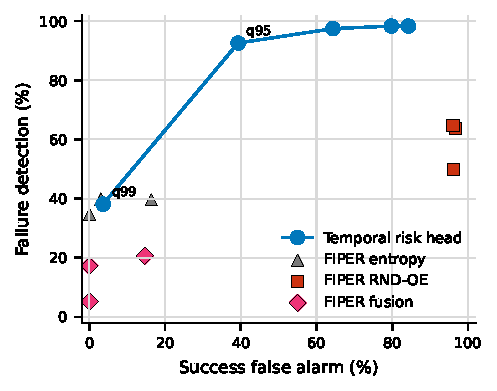
\includegraphics[width=\columnwidth]{figures/fig_results_seen_calibrated_ood_transfer.pdf}
  \caption{Seen-calibrated monitor transfer to six unseen suites. Each point is
  computed on the same 331 successful and 349 failed episodes. The temporal
  risk-head curve varies only thresholds fixed on seen data; the three points
  per FIPER family are its CT-quantile, TVT-quantile and TVT-CP-band rules.
  Neither method is recalibrated on the OOD outcomes.}
  \label{fig:detector-transfer}
\end{figure}

\subsection{Matched LIBERO-PRO evaluation}

Table~\ref{tab:libero-pro-main} and Fig.~\ref{fig:libero-pro-success} report
2,000 matched episodes per policy. U-VOWEL with the explicit latch-50 controller
reaches 888/2,000 successes (44.40\%), compared with 836/2,000 (41.80\%) for
SimVLA and 812/2,000 (40.60\%) for the world model. The absolute gains are 52
and 76 episodes, respectively. They are concentrated in Goal-Language and
Goal-Object. All policies remain weak on Goal-Swap and Goal-Task, where routing
cannot recover a capability absent from both branches.

\begin{table*}[t]
  \caption{Matched official LIBERO-PRO success. Each suite contains 500
  episodes (10 tasks, 50 initial states per task); Overall contains 2,000
  episodes. Bold marks the best result in each column.}
  \label{tab:libero-pro-main}
  \centering
  \small
  \begin{tabular}{lccccc}
    \toprule
    Policy & Goal-Language & Goal-Object & Goal-Swap & Goal-Task & Overall \\
    \midrule
    World model H10 & 387 (77.4\%) & 352 (70.4\%) & \textbf{25 (5.0\%)} & \textbf{48 (9.6\%)} & 812 (40.60\%) \\
    HF SimVLA H10 & 397 (79.4\%) & 406 (81.2\%) & 20 (4.0\%) & 13 (2.6\%) & 836 (41.80\%) \\
    Fresh U-VOWEL & \textbf{410 (82.0\%)} & 415 (83.0\%) & 18 (3.6\%) & 42 (8.4\%) & 885 (44.25\%) \\
    \textbf{Latch-50 U-VOWEL} & 408 (81.6\%) & \textbf{423 (84.6\%)} & 16 (3.2\%) & 41 (8.2\%) & \textbf{888 (44.40\%)} \\
    \bottomrule
  \end{tabular}
\end{table*}

\begin{figure*}[t]
  \centering
  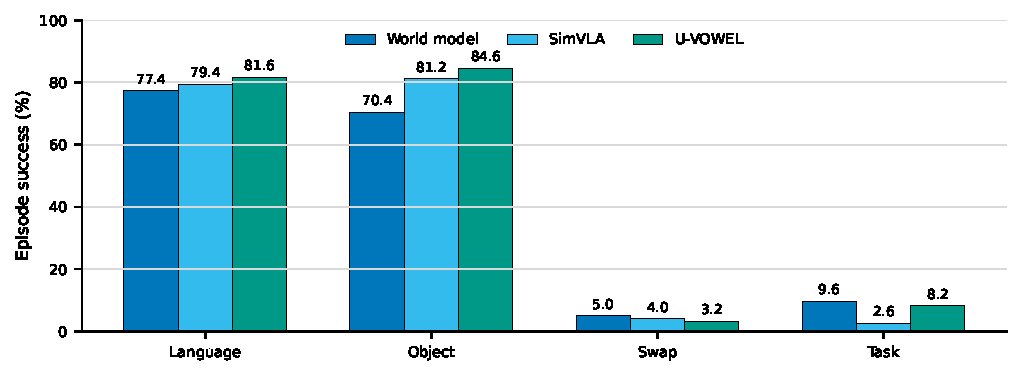
\includegraphics[width=0.93\textwidth]{figures/fig_results_libero_pro_success.pdf}
  \caption{Suite-level success on matched official LIBERO-PRO episodes. The
  selected U-VOWEL controller improves the aggregate result through the
  Language and Object suites, but does not solve the Swap or Task shifts.}
  \label{fig:libero-pro-success}
\end{figure*}

The paired outcomes in Table~\ref{tab:paired-outcomes} confirm that the branches
are complementary rather than nested. Relative to SimVLA, U-VOWEL gains 149
episodes and loses 97 (exact McNemar \(p=0.00110\)); relative to the world
model, it gains 207 and loses 131 (\(p=0.00004\)). Fresh re-query and latch-50
are statistically indistinguishable on this manifest (\(p=0.79137\)), which
supports selecting the latch by compute rather than by a success claim. These
tests are descriptive: the evaluation uses one seed and repeated initial states
nested within tasks.

\begin{table}[t]
  \caption{Paired official LIBERO-PRO outcomes for latch-50 U-VOWEL.}
  \label{tab:paired-outcomes}
  \centering
  \footnotesize
  \setlength{\tabcolsep}{3.2pt}
  \begin{tabular}{lrrrrr}
    \toprule
    Comparator & Both & U only & C only & Neither & \(p\) \\
    \midrule
    World model & 681 & 207 & 131 & 981 & 0.00004 \\
    SimVLA & 739 & 149 & 97 & 1,015 & 0.00110 \\
    Fresh U-VOWEL & 858 & 30 & 27 & 1,085 & 0.79137 \\
    \bottomrule
  \end{tabular}
\end{table}

On the separate project-specific Goal-Object-OOD protocol, the same ranking is
observed over 900 matched episodes: 823 successes for the world model (91.44\%),
841 for SimVLA (93.44\%), 859 for fresh re-query (95.44\%) and 861 for latch-50
U-VOWEL (95.67\%). We keep this result separate because this 18-task suite is
not an official LIBERO-PRO benchmark.

\subsection{Success--compute trade-off}

Fresh re-query invokes the world model 32,883 times on the official protocol.
The 50-action latch reduces this to 6,761 checks, a 79.4\% reduction, while
recording three additional successes. Of those checks, 2,940 world-model
proposals are accepted and 3,821 are rejected; the latch bypasses 27,251
otherwise eligible checks. As shown in Fig.~\ref{fig:success-compute}, the
selected controller therefore retains the fused policy's success level while
reducing successful-episode time from 14.11 to 7.35\,s. It remains slower than
standalone SimVLA (2.69\,s), but faster than the standalone world model
(14.16\,s).

\begin{figure}[t]
  \centering
  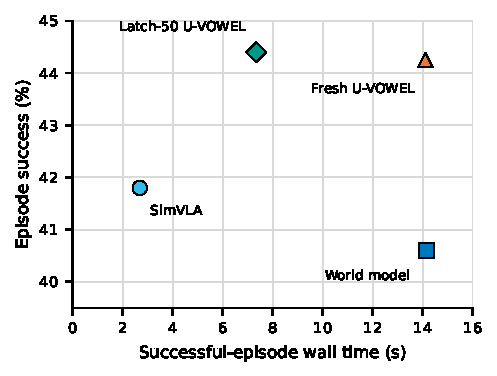
\includegraphics[width=\columnwidth]{figures/fig_results_success_compute.pdf}
  \caption{Official LIBERO-PRO success versus measured wall time on successful
  episodes. The latch improves the compute profile of fresh routing without a
  measurable success difference on the matched manifest.}
  \label{fig:success-compute}
\end{figure}

\subsection{Risk-monitor transfer across VLA backbones}

Table~\ref{tab:cross-backbone} summarizes the completed online VLA-only
ablations. These rows test portability, not a shared leaderboard: the
backbones, feature availability, controller rules and episode manifests differ.
The SimVLA six-suite replay gains 11 successes under risk-guided candidate
selection. OpenVLA gains 38 successes over H8 when risk controls execution
horizon, but its fixed-H1 control reaches 1,022/1,800 (56.78\%) and therefore
outperforms the adaptive policy. Pi0.5 gains five episodes on Goal-Swap yet
loses 18 on OOD18, where the base policy already succeeds on 97.44\% of
episodes. These mixed outcomes show that offline warning quality does not by
itself guarantee beneficial online intervention.

\begin{table*}[t]
  \caption{Completed cross-backbone online ablations. Results are internally
  matched within each row but not comparable across rows.}
  \label{tab:cross-backbone}
  \centering
  \small
  \begin{tabular}{llllr}
    \toprule
    Backbone and protocol & Reference policy & Risk-aware policy & Successes & Change \\
    \midrule
    SimVLA, six-suite replay & Original H10 & Candidate argmin-cap H10 & 392/680 \(\rightarrow\) 403/680 & +11 \\
    OpenVLA, Goal-Object-OOD & Fixed H8 & Adaptive H1/H8 & 976/1,800 \(\rightarrow\) 1,014/1,800 & +38 \\
    Pi0.5, official Goal-Swap & Basic H10 & Selected-cap H10 & 161/500 \(\rightarrow\) 166/500 & +5 \\
    Pi0.5, official OOD18 & Basic H10 & Selected-cap H10 & 1,754/1,800 \(\rightarrow\) 1,736/1,800 & -18 \\
    \bottomrule
  \end{tabular}
\end{table*}

% IsaacLab and physical-robot results are intentionally omitted until the
% corrected H10 and matched hardware protocols have completed. No interim H1
% collection or unmatched physical result is used in this paper version.
